%%%%%%%%%%%%%%%%%%%%%%%%%%%%%%%%%%%%%%%%%%%%%%%%%%%%%%%%%%%%%%%%%%%%%%%%%%%%%%
%%%%%%%%%%%%%%%%%%%%%%%%%%%%%%%%%%%%%%%%%%%%%%%%%%%%%%%%%%%%%%%%%%%%%%%%%%%%%%
%%
%%%%%%%%%%%%%%%%%%%%%%%%%%%%%%%%%%%%%%%%%%%%%%%%%%%%%%%%%%%%%%%%%%%%%%%%%%%%%%
%%%%%%%%%%%%%%%%%%%%%%%%%%%%%%%%%%%%%%%%%%%%%%%%%%%%%%%%%%%%%%%%%%%%%%%%%%%%%%
\documentclass[12pt,a4paper,titlepage,final]{article}
\newcommand{\uv}[1]{\quotedblbase #1\textquotedblleft}
% cestina a fonty
\usepackage[czech]{babel}
\usepackage[utf8]{inputenc}
% balicky pro odkazy
\usepackage[bookmarksopen,colorlinks,plainpages=false,urlcolor=blue,unicode]{hyperref}
\usepackage{url}
% obrazky
\usepackage[dvipdf]{graphicx}
\usepackage{listings} 
% velikost stranky
\usepackage{graphicx}
\usepackage[top=3.5cm, left=2.5cm, text={17cm, 24cm}, ignorefoot]{geometry}

\begin{document}

\begin{titlepage}

\begin{figure}[h]
\begin{center}

\includegraphics[scale=0.6]{logo.eps}
\end{center}
\end{figure}

\begin{center}
\LARGE
\textsc{Vysoké učení
  technické v~Brně\\ \Large{Fakulta informačních technológií}}\\
\vspace{\stretch{0.382}}
\LARGE
SHO Štátna volebná infraštruktúra \\
\Huge
Dokumentácia z predmetu IMS\\ 
\large{\medskip
\today }\\
\vspace{\stretch{0.618}}
\end{center}
 \hfill   

\begin{flushleft}
\begin{large}
\begin{tabular}{ll}
\textbf{Autori:} \\ \\

Martin Maga  xmagam00, \\Vojtěch Meca   xmecav00 \\ \\


\end{tabular}
\end{large}
\end{flushleft}
\end{titlepage}


\tableofcontents
\newpage

\section{Úvod}
Táto dokumentácia sa zaoberá vývojom, implementáciou a testovaním systému hromadnej obsluhy "Štátna volebná infraštruktúra", ktorá simuluje\cite{Kutis:Simulace} volebný systém v Českej republike zahrňujúci voľby v okrskov a krajských mestskách a následne odoslanie a počítanie hlasov v informačnom centre.\\

Na základe modelu a simulácie bude ukázané chovanie systému so zreteľom na ukázanie slabých miest pri voľbách. Tento projekt môže byť použitý na optimalizáciu systému voliev v Českej republike vzhľadom na zrýchlenie celého systému počítania hlasov a rozdelenia do okrskov.

\subsection{Autori}
Na projekte SHO "Štátna volebná infraštruktúra" sa podieľali nasledujúci autori:
\begin{itemize}
\item Martin Maga(xmagam00)
\item Vojtěch Meca(xmecav00)
\end{itemize}

Okrem vyššie spomenutých ľudí sme využili možňosť konzultácie s pánom doktorom \\ Hrubým(konzultácia ohľadne správnostinášho návrhu Petriho siete).

\subsection{Zdroj informácií}
Informácie o štátnej volebnej infraštruktúre boli zisťované z dostupnej literatúry. Rovnako sme využili informácii dostupné na internete, ohľadne počtu okrskov a ich voličov. Rovnako sme využili štatistiky, ktoré sme generovali pri skončení programu.


  


\subsection{Testovacie prostredie}
Pre testovacie účely boli použité architekrúry:Linux 3.2.0-56-generic $86_64$ GNU/Linux pre menšie vzorky dát a pre rozsiahlejšie testovanie na väčšej vzorke dát: FreeBSD eva.fit.vutbr.cz 9.2-STABLE FreeBSD amd64.

\subsection{Validita}
Experimentovaním sme overovali validitu modelu, ktoré vo forme štatistik a jeho následnej analýze odpovedali nášhu odhadovanému predpokladu. Tak isto sme využili dostupné informácie o spôsobe volieb v Českej republiky a štatistických informáciách, ktoré sú verejne prístupné na internete.

\newpage


\subsection{Ciele projektu}
Ciele projektu zahŕňajú:
\begin{itemize}
\item Analýza aktuálneho volebného systému v Českej republike
\item Analýza slabých miest volebného systému
\item Návrh efektívnejšieho prístupu, ktoré by dokázalo zvýšiť rýchlosť počítania hlasov
\item Návrh co nejvíce reálného systému voleb v České republice 
\end{itemize}


\section{Rozber témy a použitých technológií}

\indent

\subsection{Téma práce}
Témou práce bola implementácia systému hromadnej obsluhy štátnej volebnej infraštruktúry. Volebná infraštruktúra v Českej republike funguje na nasledovnom princípe:
Česká republika sa zaraďuje medzi dvojkomorové parlamentné 
systémy. Tvorí ju Poslanecká snemovňa a Senát. Do PS ČR sa volí na 
základe pomerného voličského systému.  Ďalším dôleţitým zákonom je 
zákon č. 247/1995 Sb., o voľbách. Tieto právne pramene sú základnými právnymi 
prameňmi v oblasti volieb v ČR.\cite{Seda:Voleb}

Voľby prebiehajú štandardne každé 4 roky, alebo po predčasných voľbách. Každému občanovi republiky prislúcha 1 volebný hlas, ktorý musí odovzdať. Každý občas patrí pod istý volebný kraj, ktorý sa delí na menšiu časti zvané okrsky. Voľby prebiehajú štandardne v sobotu alebo v nedeľu dokopy 14 hodín. Každý občan, ktorý spĺňa podmienky príde v mieste svojho bydliska do volebnej miestnosti, kde sa preukáže platnosti dokladom totožnosti volebnej komisii, ktorá skontroluje údaje a povolí občanovi voliť. Každý občan ide jednotlivo za urnu, kde zaškrtne možnosť a následne vhodí svoj hlas do urny a zvyšné zahadzuje.

Na konci volieb sú hlasí v jednotlivých okrskoch sčítané a odnesené na obecný úrad, odkiaľ sa posielalu na prepočítanie do volebného centra.

  


\subsection{Popis použitých postupov}
Systém je simulovaný pomocou diskrétnej simulácie (předmet IMS slajd 122) ako systém hromadnej obsluhy 
(předmet IMS slajd 139). Je to výhodné napr. z hľadiska sledovania dĺžky front (predmet IMS slajd 141) 
obslužných liniek (predmet IMS slajd 139) jednotlivých častí volebného centra. Použitou 
technologií k tomuto účelu je jazyk C++ a knižnica Simlib (predmět IMS (1) slajd 72). Výhodou spomínaných 
technológií je  rýchlosť simulácie.



\subsection{Pôvod použitých technológií}
\begin{itemize}
\item Simlib -http://www.fit.vutbr.cz/~peringer/SIMLIB/ (GNU LGPL)
\item C++ - http://en.wikipedia.org/wiki/C++
\item Ubuntu - http://www.ubuntu.com/
\item Petriho siete - $http://en.wikipedia.org/wiki/Petri_net$

\end{itemize}










\section{Koncepce - modelářska témata}
V tejto kapitelo bude načrtnutý koncetuálny model predstavujúci systém volebnej infraštruktúry.
Na obrázku č. \ref{koncept} je uvedeno schéma systému Volební infrastruktury. 
\begin{figure}[h]

\begin{center}

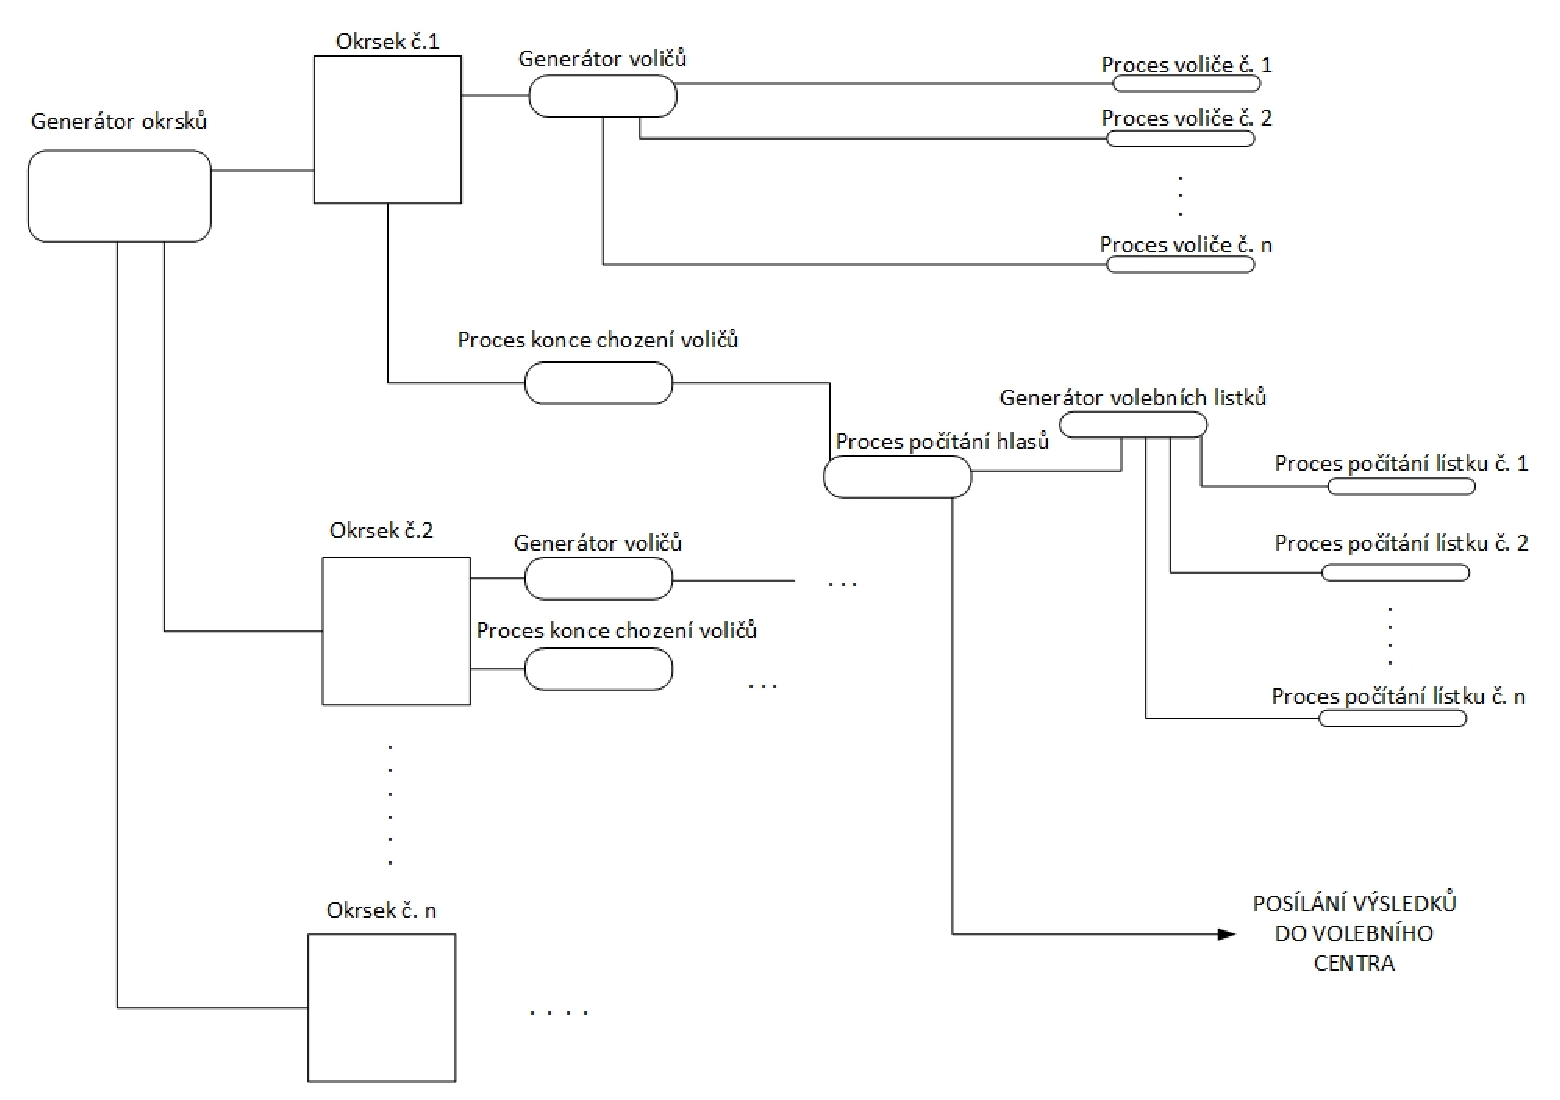
\includegraphics[scale=0.7]{img/konceptualni_model.eps} 
\caption{Konceptuálny model}
\label{koncept}

\end{center}

\end{figure}
\newpage

\subsection{Opis konceptuálneho modelu}
 V obrázku č. \ref{koncept}můžeme vidět několik různých obdelníčků a zaoblených obdelníčků. Popišeme si je jednotlivě: 
 \begin{itemize}
\item    a) Zaoblený obdelníček s názvem Generátor okrsků
\subitem  Tento zaoblený obdelníček má za úkol generovat obdelníčky Okrsky. Generuje jich přesně kolik jich má vzniknout (určeno například souborem). Po vygenerovaní Okrsků generátor ukončí svou činnost.
\item    b) Normální obdelníček s názvem Okrsek č. 1...n
\subitem  Při vytvoření tohoto objektu  se nainicialzují hodnoty, které jsou získány z Generátoru okrsků a dále vytvoří si Generátor voličů a taktéž si vytvoří Proces konce chození voličů. Poté objekt slouží pouze pro ukládání hodnot, které se můžou během programu měnit.
\item    c) Zaoblený obdelníček s názvem Generátor voličů
\subitem  Po vytvoření Okrsekem začne generovat voliče, kteří jdou volit. Vytvoří jich podle parametru maximálního počtu voličů a dále taky podle parametru volební účast voličů. Po vygenerovaní všech voličů, zahlásí konec voleb, a tímto její činnost skončí. 
\item    d) Zaoblený obdelníček s názvem Proces voliče č. 1 .. n
\subitem  Je vytvořen Generátorem voličů. Po vytvoření simuluje všechny zásadní pokyny po správné odvolení voliče. Po samotném odvolení voliče proces končí.
 \item   e) Zaoblený obdelníček s názvem Proces konce chození voličů
\subitem  Je vytvořen Okrskem. Zapne v sobě časovač reprezentující dobu voleb. Po uplynutí časovače nebo po příchodu všech voličů v okrsku se vyvolá Proces počítání hlasů. Poté jeho činnost končí.
\item    f) Zaoblený obdelníček s názvem Proces počítání hlasů
\subitem  Vytváří Genreátor volibních lístků. Správně spočítáné výsledky posílá do Volebního centra. Poté jeho činnost končí.
\item    g) Zaoblený obdelníček s názvem Proces generátor volebních lístků
\subitem  Po vytvoření Procesem počítání hlasů začne generovat Procesy počítání listků č.1 .. n. Po vygerenerování všech lístků zkončí svou činnost.
\item    h) Zaoblený obdelníček s názvem Proces počítání listků č.1 .. n
\subitem  Po vytvoření simuluje práci jednoho člena volební komise s tímto lístkem. Po ukončení počítání tohoto lístku jedním členem komise činnost tohoto obdelníčku končí.
\end{itemize}\newpage 
\subsection{Ukážka Petriho siete pre odovzdávanie hlasu}

\begin{figure}[h]

\begin{center}

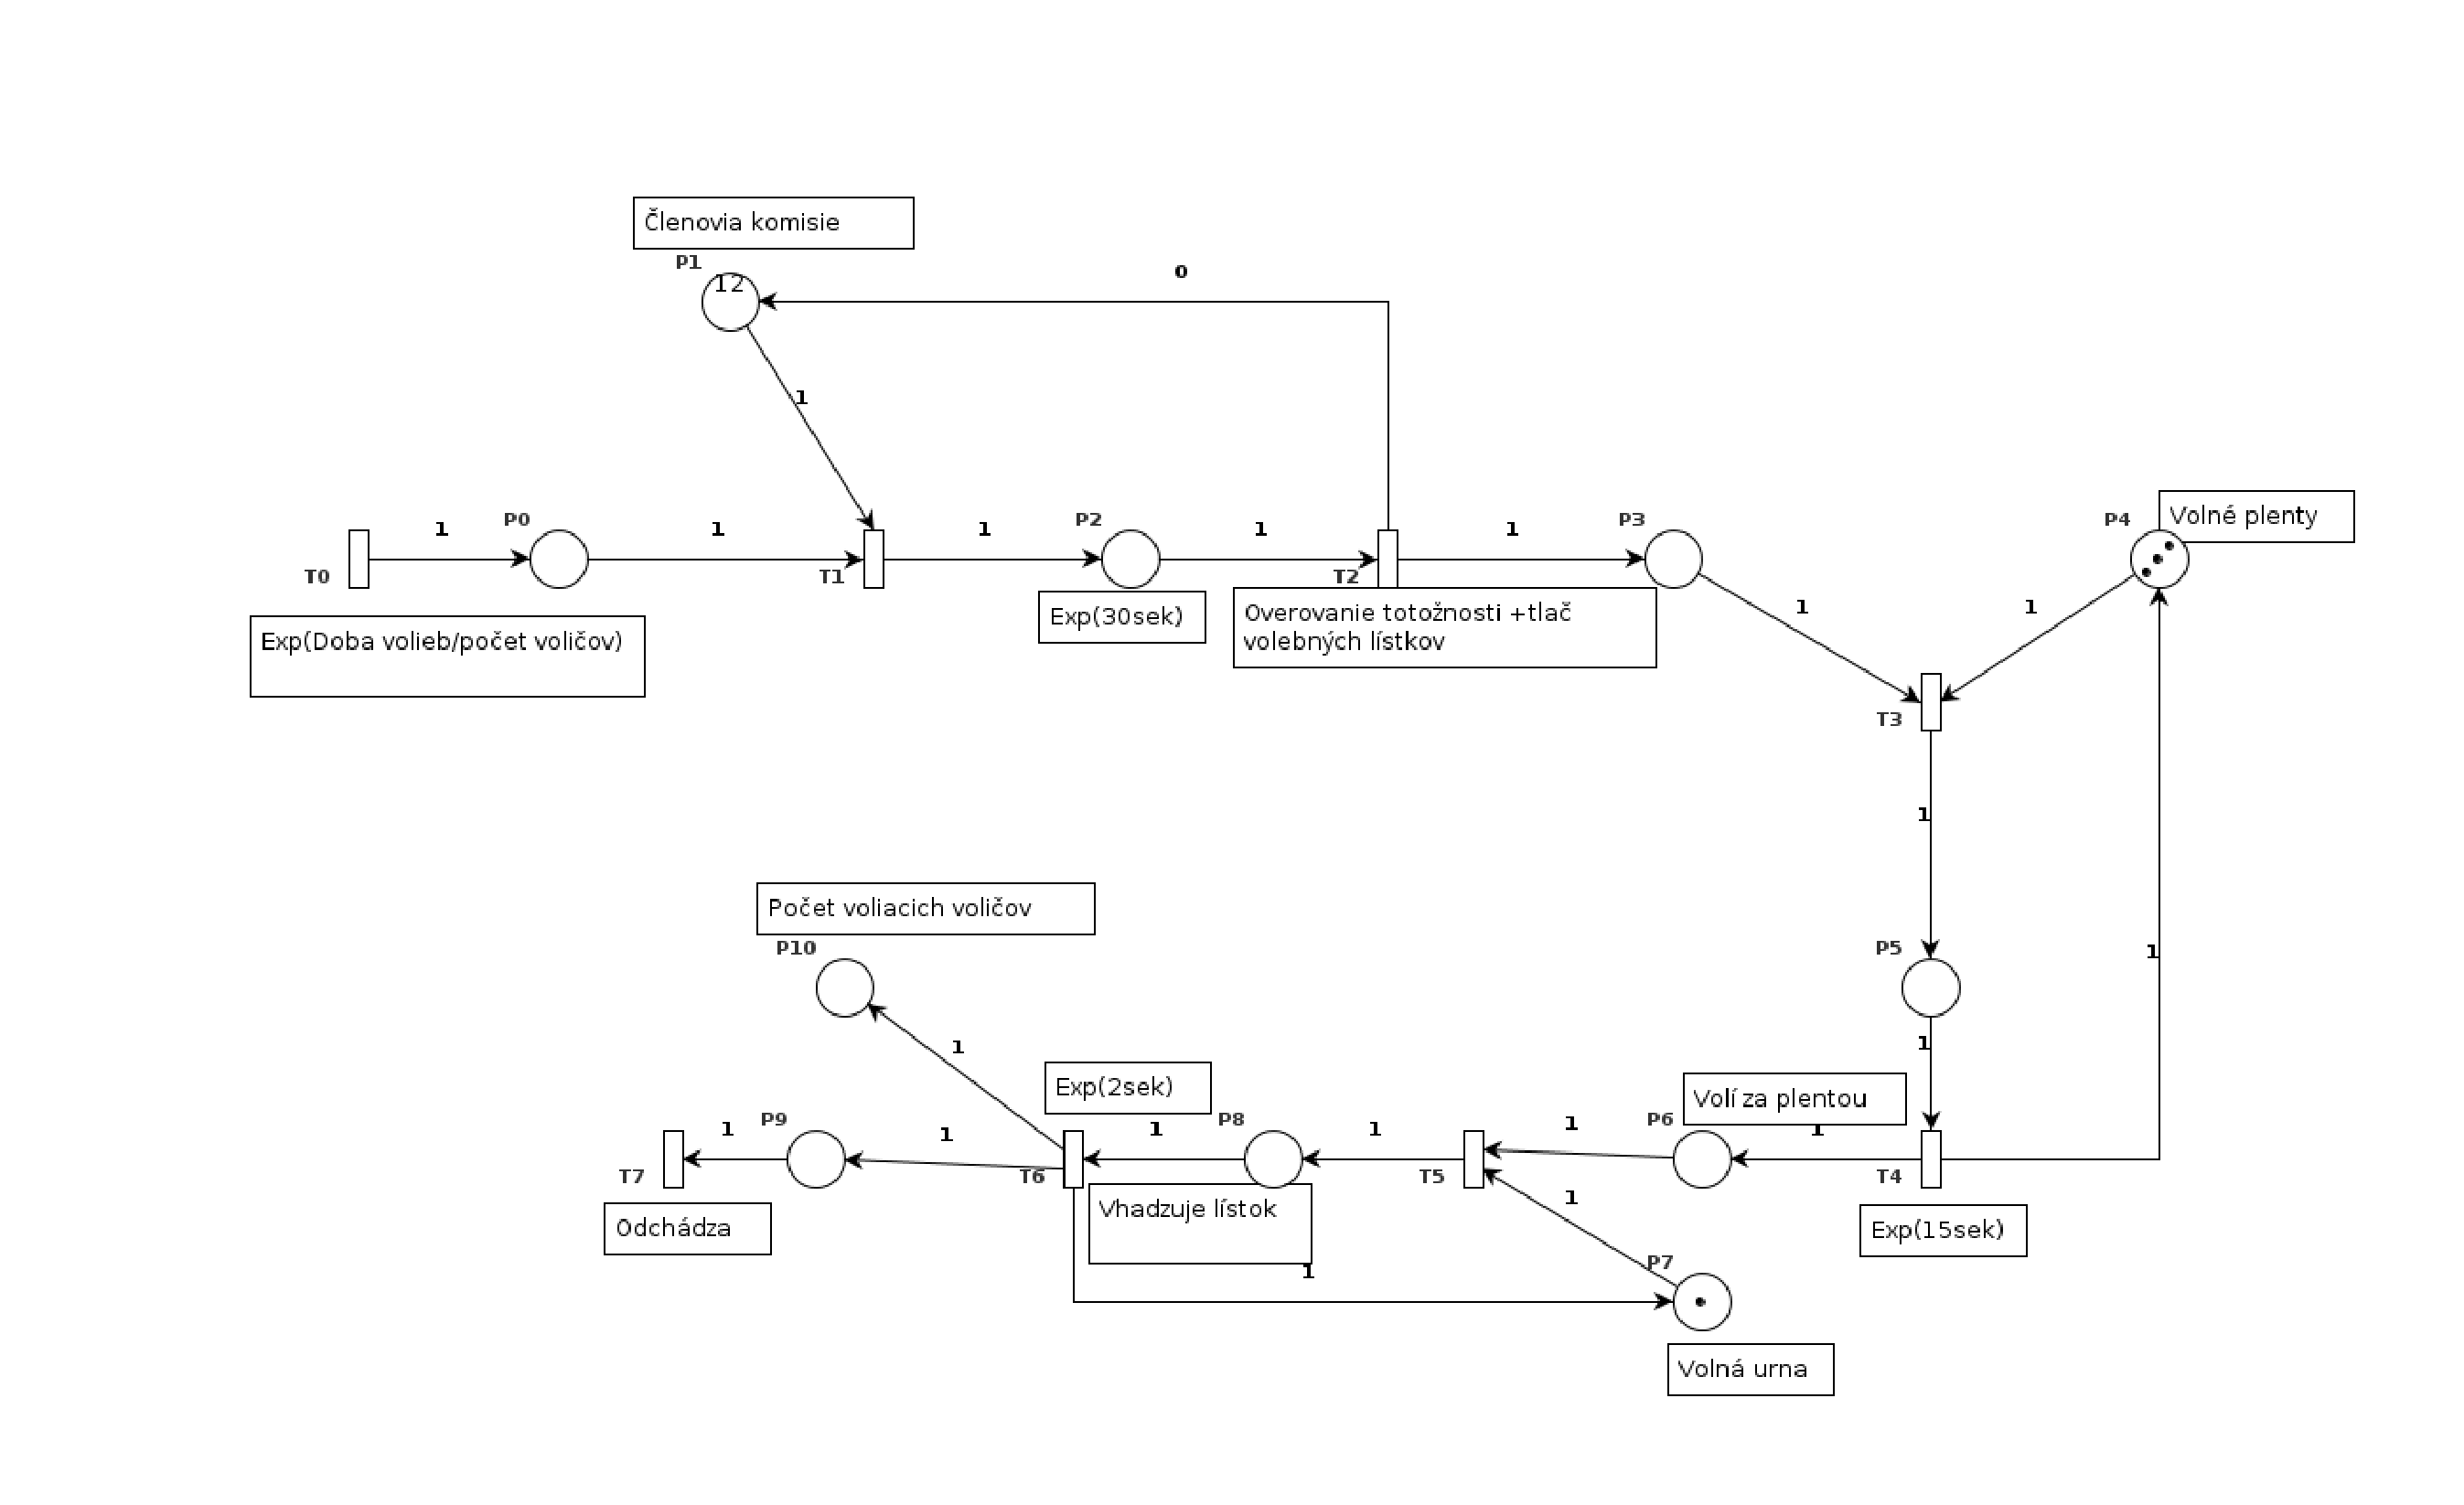
\includegraphics[scale=0.4]{img/petri2.eps} 
\caption{Petriho sieť pre odovzdávanie hlasu}
\label{petri}

\end{center}

\end{figure}

Obrázok č.\ref{petri} popisuje Petriho sieť, ktorá ukazujem systém volieb. Ukazuje príchod voliča, odvolenie voliča. Na začiatku sa vygenerujú voliči, ktorí prijdu do volebnej miestnosti. Pri vstupe do miestnosti si občan zabere člena volebnej komisie, ktorý je reprezentovaný štruktúrou "Store" s kapacitou 12 v Simlibe. \\ Pokiaľ nie je voľný nejaký člen volebnej komisie, tak se zařadí do společné fronty a čeká na uvolnění některého ze členů volební komise. Pokiaľ sa občan dostane na radu, tak ho člen volebnej komisie skontroluje. To trvá exponeniciálně 30 sekúnd. Po skončení kontroly občana členem volební komise, občan pokračuje ďalej. Zabere si "Store" s kapacitou 3, ktorý reprezentuje volebnú plentu. \\ V prípade, že nie je volná plenta, tak sa občan zaradí do jedné společné fronty. Následne užívateľ zajde za plentu a zaškrtá výsledok. To trvá exponenciálně 15 sekúnd. Následne si zabere plentu, ktorá je len 1. Pokiaľ nie je voľná tak sa zaradí do fronty a čaká. Po vhození lístku reprezentující dobu exponenciálně 2 sekundy občan opúšťa systém.
\newpage





\subsection{Implementácia}
Program pracuje na základním procesu, který regeneruje v čase nula objekty reprezentující okrsky České republiky. Při vytvoření objektu jednotlivého okrsku se nainicializují data. Objekt reprezentující okresek po inicializaci spustí po sobě jdoucí 2 procesy. První z nich je proces, který po svém vzniku začne generovat procesy příchodů voličů do volební místnosti. Druhý z procesů vytvoří časovač, který udává legální délku voleb. Po uplynutí určeného času na příchod voličů tento proces vytvoří nový proces. Nově vytvořený proces se stará o počítání jednotlivých volebních lístků ve volební místnosti, dále simuluje kontrolu výsledků a taky posílání správně vypočtených výsledků do Volebního centra České Republiky. Problém počítání jednotlivých volebních lístků řeší pomocí procesu na generování procesu počítání volebního lístku. V případě, že po spočítání výsledků se zjistí, že nastala chyba v počtech, proces zopakuje počítání volebních lístků znovu. 


\section{Architektura simulačního modelu}

\subsection{Zmena implementácie v knižnici SimLib}
Při kompilaci modelu jsme narazili na problém v knihovně SimLib konkrétně s proměnou CANARY1. Po konzultaci s Dr. Petrem Peringerem jsme změnili v knihovně SimLib v souboru process.cc řádek 405 \textbf{volatile int mylocal = CANARY1;} na řádek \textbf{volatile long mylocal = CANARY1;}. Tím se problém vyřešil a náš model jsme mohli zkompilovat.

\subsection{Okrsky navrhnuté k simulácií}
Data k okrskům jsme získávali při experimentech ze souboru \textbf{okrsky.txt}. Na prvním řádku získáváme informaci o množství okrsků. Další řádky jsou ve formátu 4 posobě jdoucích informací. První z nich je číslo kraje. Druhý z nich je název kraje, další údaj v sobě nese název krajského města. Pokud kraj nemá krajské město, tak zde nacházíme znak \textbf{'-'}. Poslední a nejduležitější je údaj o počtu občanů v okrsku.

\subsection{Popis architektury}
Simulační model má za zálkadní jednotku minutu. \newline
V programu je několik tříd, které zajišťují jeho spávný průběh. 
 \begin{itemize}
\item Třída GenOkrsku
\subitem Tato třída reprezentuje proces Generování okrsku z konceptuálního modelu na Obr. č. 1. Tato třída se dědí od třídy Event z knihovny SIMlib obsahuje pouze jednu metodu Behavior(). Metoda Behavior() ze začátku načítá první řádek ze souboru. V souboru na prvním řádku je informace o celkovém počtu okrsků. Dále pokračuje jedním cyklem, který při každém průchodu načítá data jednoho řádku ze souboru, což reprezentuje data určené právě pro jeden okrsek. Poté cyklus pokračuje vytvořením nového oběktu třídy Okrsek a posílá získané data ze souboru do jako parametry konstruktoru. Po vytvoření všech Oksrku, svou činnost končí.

\item Třída Okrsek
\subitem Tato třída reprezentuje objěkt Okrsek z konceptuálního modelu na Obr. č. 1. Tato třída má konstruktor a mnoho dalších metod na získávání, nastavování atributů třídy. Také tato třída obsahuje metody, které inkrementují nebo dekterentují některé atributy třídy. Třída je určena jako ukládání a uchovávání dat se kterými se během programu pracuje. V konstruktoru nainicializuje potřebné atributy. A po té vytvoří proces GenVolicu a předá mu parametr, jako ukazatele na sebe (pomocí ukazatele this). Poté vytváří podobně jako před tím další proces TimerVoleb. Předává mu do kontruktoru také ukazatel na sebe. Tím končí konstruktor této třídy.

\item Třída GenVolicu
\subitem Tato třída reprezentuje proces Generování voličů z konceptuálního modelu na Obr. č. 1. Tato třída se dědí od třídy Event z knihovny SIMlib a obsahuje konstruktor a metordu Behavior(). V konstruktoru se předá ukazatel z objěktu Okrsku ze kterého byl generátor vytvořen do svojeho atributu třídy Okrsku. Dále se taky zde definuje čas, který slouži pro znovu aktivovaní této třídy. Zde také měníme parametr účast volíčů pro celou ČR. V mětodě Behavior() se testuje jestli nenastal konec voleb. Zda-li nenastal, tak vytvoří objekt procesu voliče a předá mu parametr objektu Okrsek, ze kterého byla tato třída vytvořena. Inkrementuje počet generovaných voličů v okrsku a testuje jestli počet vygenerovaných voličů se rovná maximálního počtu voličů v daném okrsku, což je uloženo v atributu Okrsku s názvem pocet\_volicu. Pokud bylo vytvořeno méně voličů, tak se znovu tato třída aktivuje podle součtu času Time a času určeného v konsturuktoru. Ale pokud je vytvořeno stejně voličů jako maximální počet, tak se tato třída znovu neaktivuje, ale nastaví parametr end\_voleb třídy Okrsku na 1 a to pomocí metody konec\_voleb() v objektu Okrsek a tím ukončí dobu konce voleb daného okrsku. 

\item Třída Volic
\subitem Tato třída reprezentuje Proces voliče z konceptuálního modelu na Obr. č. 1. Tato třída se dědí od třídy Process z knihovny SIMlib a obsahuje konstruktor a metordu Behavior(). V konstruktoru se předá ukazatel z atributu okrsek třídy GenVoličů, ve kterém je uložen ukazatel na konkrétní okrsek. Metoda Behavior() určuje chování voliče ve volební komisi. Při vstupu voliče se nejprve zvýší číslo aktuálních voličů v místnoti o 1 pomocí metody v objektu Okrsku increment\_lidi\_v\_mistnosti(). Poté proces voliče pokračuje zabráním si jednoho člena komise, reprezentujícího Store s názvem komise pomocí metody get\_komise() z objektu Okrsek. Po uplynutí dané doby pomocí SIMlib funkce Wait() uvolní zabraného člena komise. Podobně si zabere i jednu z plent. Planta je taky typu Store. Nakonec podobně jako předchozí zařízení zabere i urnu, která je reprezentována zařízením Facility. Proces skončí po odečtení aktuálního čísla voličů pomocí metody decrement\_lidi\_v\_mistnosti().

\item Třída TimerVoleb
\subitem Tato třída reprezentuje Proces konce chození voličů z konceptuálního modelu na Obr. č. 1. Třída je určena pro ukončení voleb po uplynutí celkového času voleb. Tato třída se dědí od třídy Process z knihovny SIMlib a obsahuje konstruktor a metordu Behavior(). V konstruktoru se předá ukazatel z objěktu Okrsku ze kterého byl timer vytvořen do svojeho atributu třídy Okrsku. V metodě Behavior() se zpustí cyklus, který reprezentuje dobu voleb příchodu voličů způsobem, že v každém cyklu čeká minutu pomocí Wait() a testuje jestli nenastal konec voleb pomocí metody třídy Okrsek get\_konec\_voleb(). Poté spustí cyklus, který čeká na uvolnění místnosti od všech voličů. Testuje se atribut lide\_v\_mistnosti třídy Okrsek. Před ukončením svého konání proces TimerVoleb vytvoří nový proces s názvem PocitaniHlasu a předá mu ukazatel na objekt Okrsku, ze kterého byl vytvořen a aktivuje ho.

\item Třída GenHlasu
\subitem Tato třída reprezentuje Generátor volebních lístků z konceptuálního modelu na Obr. č. 1. Tato třída se dědí od třídy Event z knihovny SIMlib a obsahuje konstruktor a metordu Behavior(). V konstruktoru se předá ukazatel z atributu okr třídy TimerVoleb, ve kterém je uložen ukazatel na konkrétní okrsek. V metodě Behavior() se vytvoří proces PocitaniKonkretnihoHlasu s ukazatelem na Okrsek ulozený v atributu okr třídy a poté se aktivuje. Pomocí metody decrement\_poc\_lisktu() se sníží počet nespočtených volebních lístků. Dále se testuje jestli se vygenerovali všechny lístky pro daný okrsek pomocí metody get\_poctu\_zvolenych\_listku(). Pokud metoda vrátí 0 nastaví se atribut spoctene\_hlasy objektu Okrsku. Pokud metoda vrátí jiné číslo, znovu aktivuje se tato třída v čase Time.

\item Třída PocitaniKonkretnihoHlasu
\subitem Tato třída reprezentuje Proces počítání lístků z konceptuálního modelu na Obr. č. 1. Tato třída se dědí od třídy Process z knihovny SIMlib a obsahuje konstruktor a metordu Behavior(). V konstruktoru se předá ukazatel z atributu okr třídy GenHlasu, ve kterém je uložen ukazatel na konkrétní okrsek. Metoda Behavior() určuje chování počítání lístku členem volební komise. Při začátku počítání lístku se nejprve zvýší číslo aktuálních právě počítaných lístků o 1 pomocí metody v objektu Okrsku increment\_prave\_pocitanych\_listku(). Poté proces počítání lístku pokračuje zabráním si jednoho člena komise, reprezentujícího Store s názvem komise pomocí metody get\_komise() z objektu Okrsek. Po uplynutí dané doby pomocí SIMlib funkce Wait() uvolní zabraného člena komise. Poté vyhodnotí zda-li je lístek platný nebo neplatný. Pokud platný pomocí metody increment\_plat\_listku() v objektu Okrsek se zvýší číslo platných lístků okrsku. Zda-li je lístek neplatný použije se po zvýšení atributu poc\_nep\_listku metoda increment\_nep\_listku() v objetku Okrsek. Proces skončí po odečtení aktuálního čísla voličů pomocí metody decrement\_prave\_pocitanych\_listku().

\item Třída PocitaniHlasu
\subitem Tato třída reprezentuje Proces počítání hlasů z konceptuálního modelu na Obr. č. 1. Tato třída se dědí od třídy Process z knihovny SIMlib a obsahuje konstruktor a metordu Behavior(). V konstruktoru se předá ukazatel z atributu okr třídy TimerVoleb, ve kterém je uložen ukazatel na konkrétní okrsek. V metodě Behavior() se spustí cyklus, který testuje, zda-li má proběhnout počítání hlasů. Pokud ano, tak vytvoří proces GenHlasu a předá mu ukazatel na objekt Okrsek. Poté spustí cyklus, který končí v případě, že jsou vytvořeny všechny procesy třídy PocitaniKonkretnihoHlasu. Poté se spustí další cyklus, který kontroluje končí v případě, že jsou všechny lístky spočtené. Po nějaké době (pomocí Wait()) vyhodnotí, jestli výsledky jsou správné a nebo ne. Pokud výsledky správné nejsou, tak zavolá metodu get\_nul\_prepoctenym\_listkum(), která nastaví atributy poc\_nep\_listku a poc\_plat\_listku na 0 a atribut pocet\_zvolenych\_listku na původní hodnotu v objektu Okrsek. A cyklus pro vyhodnocení zda-li se mají výsledky počítat se spustí znovu. Pokud jsou výsledky správné, tak si proces třídy PocitaniHlasu zabere zařízení Centrum\_republiky pomocí SIMlib funkce Seize. Po uplynutí času reprezentující posílání výsledků do volebního centra republiky, se zařízení Centrum\_republiky pomocí SIMlib funkce Releise uvolní. Tím končí tento proces.

\end{itemize}


\subsection{Spustenie programu}
Pro zkompilování programu je potřeba zadat do příkazové řádky \textbf{make} v adresáři s projektem. Po úspěšném zkopilování projektu zadáme příkaz \textbf{make run}, když budeme chtít program spustit. V průběhu výpočtu programu se na obrazovku vypisují příchody a odchody jednotlivých voličů a taky začátek zpracování volebních lístků a jejich konec zpracování v jednotlivých oksrcích. Nakonec všech výpisů programu získáváme to nejdůležitější a to statistiky modelu.
\newpage


\section{Podstata simulačných experimentov}
\subsection{Postup experimentování}
Hlavní cíl, proč byl model vytvořen, bylo zjistit vytíženost Volevního celorepublikového centra a navrhnout změny pro zefektivnění vytíženosti tohoto volebního centra. Dále také jsme získávali informace o průběhu počítání hlasů pro jednotlivé kraje a pak pro celou republiku. K tomu nám pomáhali experimenty. Díky těmto experimentům jsme mohli dosáhnout validitu samotného modelu voleb. V experimentech jsme měnili parametr volební účasti, kdy jsme sledovali vytíženost volebního centra v závislosti na tomto parametru. Dále jsme takéž podle tohoto parametru sledovli, jak se chovají jednotlivé okrsky v délce počítání hlasů a v čekání na volební centrum. 
  
\subsection{Popis experimentů}
V dalších experimentech jsme se zaměřili pouze na vytíženost volebního centra. 
Vstupem byla 50\% účast voličů a očekávalo se, že výstupem bude doba čekání na volební centrum v průměru okolo 2 sekund. Z obrásku č.  \ref{50} získáme  výsledné statistiky, ve kterýc jsme zjistili, že průměrně okrsky čekají v minutách 0.0231881, což je přibližně 1.4 sekundy. Další zajímavý udaj byl, že ve frontě na volební centrum bylo maximálně 3 volební okrsky z celé republiky. Obecně se na volební centrum nečekalo. Z obrázku vidíme i další informace o výpisu statistik modelu. \newline
\newline
\begin{figure}

\begin{center}

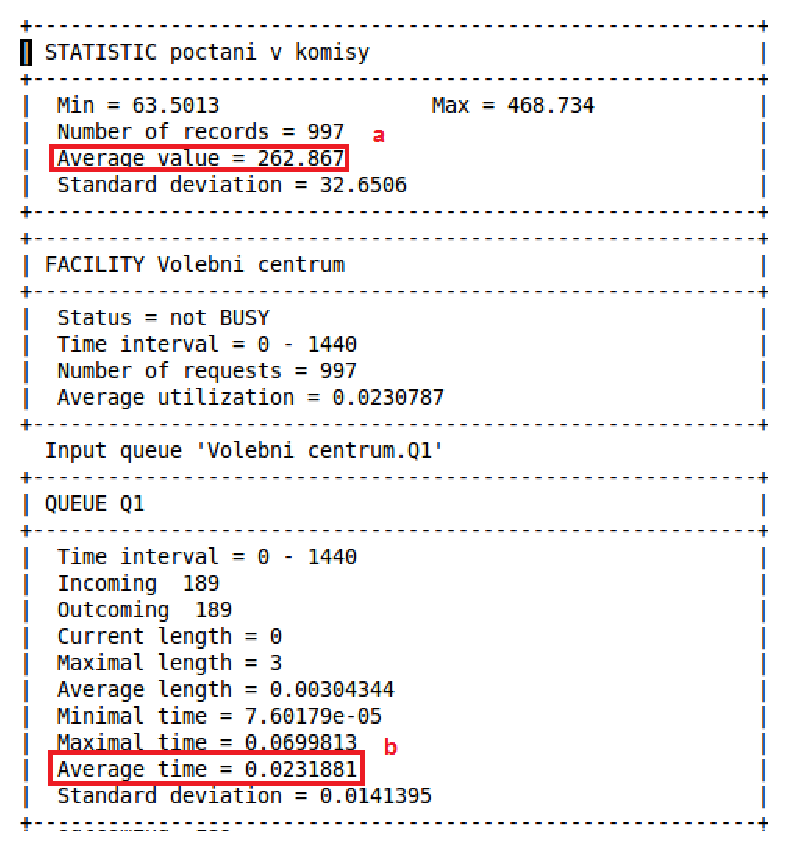
\includegraphics[scale=0.6]{img/0_5.eps} 
\caption{50\,\% účastníkov}
\label{50}

\end{center}

\end{figure}
\newline
\newline
\newpage
Dalším experimentem jsme chtěli zjistit zda-li se změní čekání okrsků na volební centrum když změníme volevní účast. Tu jsme si změnili na 175\%. Očekávali jsme delší fronty orksků na volební centrum. V obrázku č. \ref{obr3} zišťujeme výsledek, že byla změna v průměru čekání volebních okrsků byla 0.034749 v minutách, což je přibližně 2.1 sekundy. Maximální délka fronty byla 7 okrsků. \newline
\newline
\begin{figure}

\begin{center}

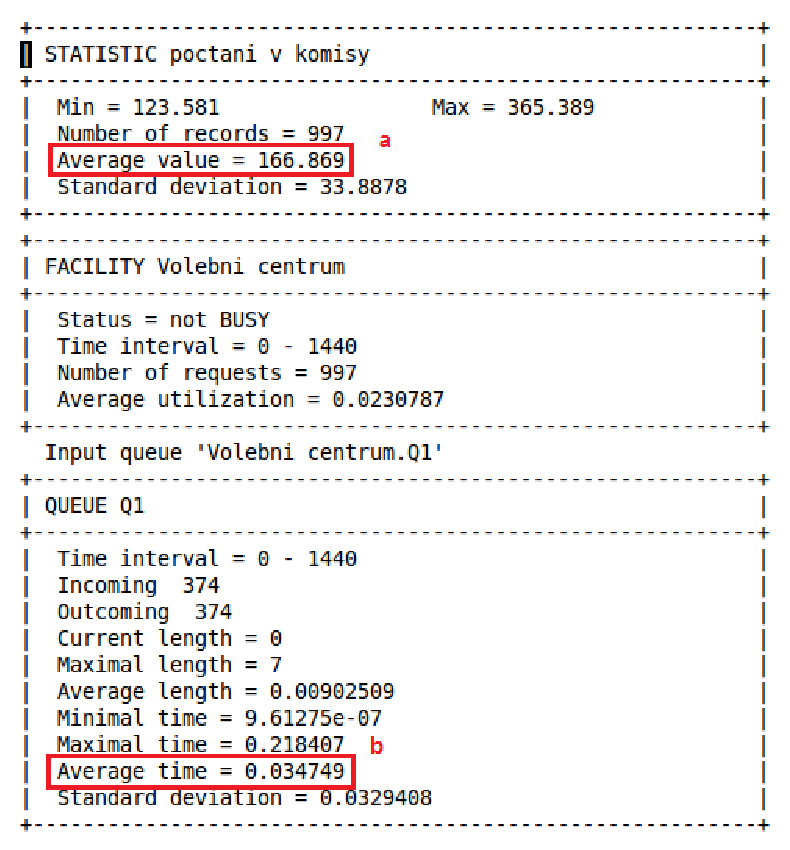
\includegraphics[scale=0.6]{img/1_75.eps} 
\caption{175\,\% účasť}
\label{obr3}

\end{center}

\end{figure}
\newpage
Toto nás dovedlo k názoru, že model volebního systému v ČR, který jsme vytvořili není tolik reálný,jak jsme zamýšleli. Změnili jsme čas zpracování výsledků na 6 sekund. A reálnost systému jsme znovu ověřovali experimentem.\ref{100}\newline
Vstupem byla 100\% účast voličů a očekávalo se, že výstupem bude doba čekání na volební centrum v průměru okolo 2-8 minut. Z obrázku \ref{102}můžeme vidět, že ve výsledných statistikách zjišťujeme, že průměrně okrsky čekají ve frontě 15 minut. Ve frontě na volební centrum se stav zlepšil na maximálních 250 volební okrsky z celé republiky. Toto byla reálnější situace, než v předchozích případech, což bylo náš cíl experimentů.
\newline
\newline
\begin{figure}[h]

\begin{center}

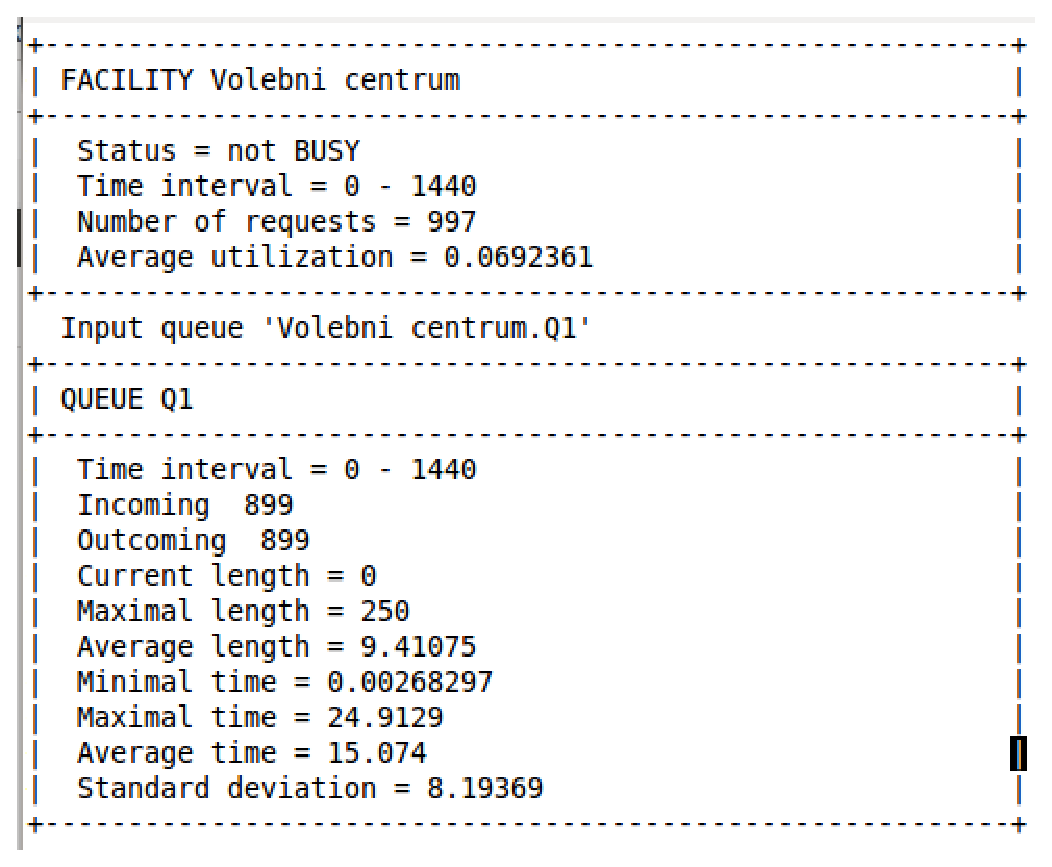
\includegraphics[scale=0.6]{img/100.eps} 
\caption{100\,\% účastníkov}
\label{100}

\end{center}

\end{figure}
\begin{figure}

\begin{center}[h]

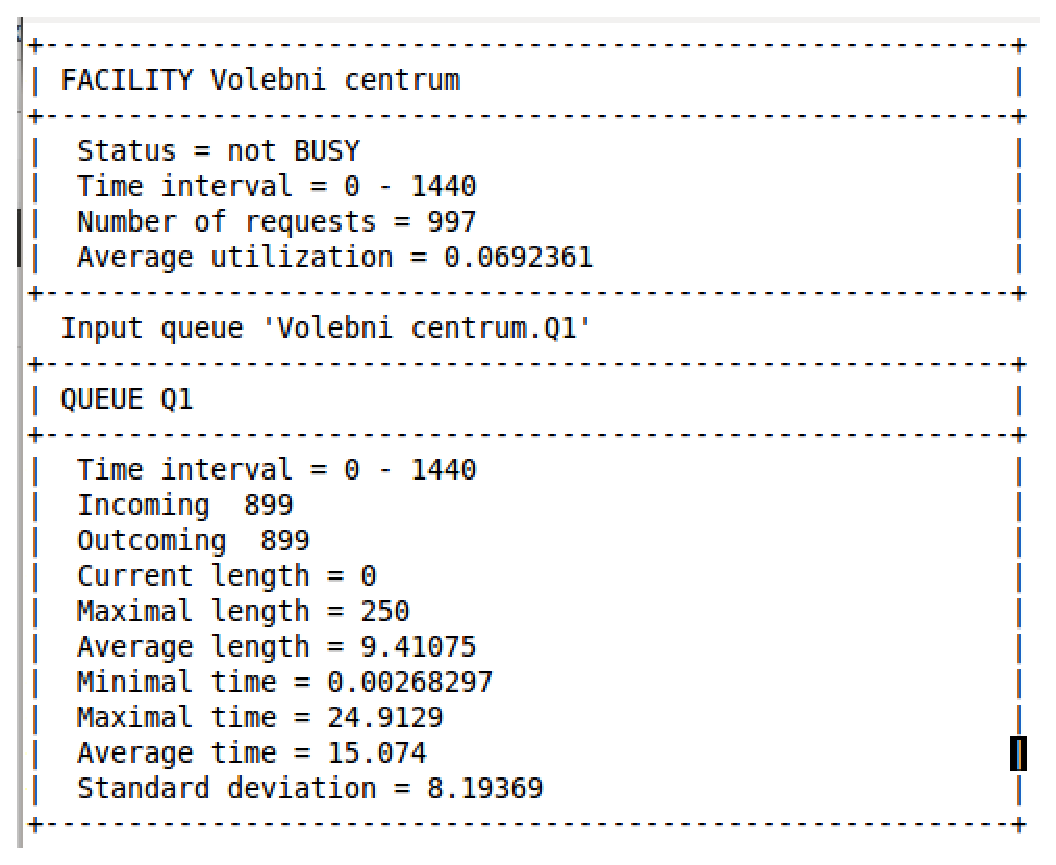
\includegraphics[scale=0.7]{img/100_second_part.eps} 
\caption{100\,\% účastníkov}
\label{102}

\end{center}

\end{figure}
\newline
\newline
\newpage
\subsection{Závěr experimentů}
Bylo provedeno 8 experimentů na vytíženost centra. V průběhů experimentů byla odstraněna nereálná situace čekání orksků na volební centrum.


\section{Zhrnutie simulačných experimentov a záver}
Naším hlavním cílem bylo vytvořit co nejvíce reálný model volebního systému. Proto jsme se striktně nerželi zadání a vyvořili jsme 997 okrsků. Také jsme zvažovali zda vytváření procesů volebních lístků je zbytečné. Ačkoli tato operace není příliš efektivní pro výpočet, pro reálnost systému je zásadní. Přístup k jednotlivým volebním lístkům je v praxi normální a proto i tento způsob v modelu jsme zachovali.\newline
Díky sadě experimentů jsme zjitili, že model je vrámci školního projektu validní.


\newpage

\section{Referencie}


\bibliographystyle{czechiso}

\bibliography{dokumentace}
\newpage
\end{document}

